% Capítulo 6
\chapter{Estudo Experimental}
\label{cap:cap6}

este capítulo consiste em apresentar o estudo por meio de método experimental, envolve a concepção do contexto do experimento, da disposição e características dos elementos envolvidos, a seleção das variáveis influenciadoras, o controle e a instrumentação do experimento, sua execução, a captura de dados durante experimentação, e por fim, a análise e conclusões obtidas a partir desses resultados. 

O objetivo do experimento é analisar a viabilidade do uso de mecanismos de \textit{throttling} como já apresentados buscando alternativa para aumentar a disponibilidade dos elementos presentes em \textit{IoT} através do ajuste de comportamento por ação de limiares de atuação que consideram seus aspectos energéticos. A abordagem é aderente aos elementos presentes na taxonomia proposta no Capítulo \ref{cap:cap4} e permite a comparação e análise entre dois dispositivos: um tendo sua operação ajustada pelo throttling e outro sem esse critério. A Figura \ref{fig:cap6metodologia} apresenta resumidamente os passos executados para realização do estudo.



\begin{figure}[H]
	\centering
	\caption{Etapas do Estudo Experimental.}
	\label{fig:cap6metodologia}
	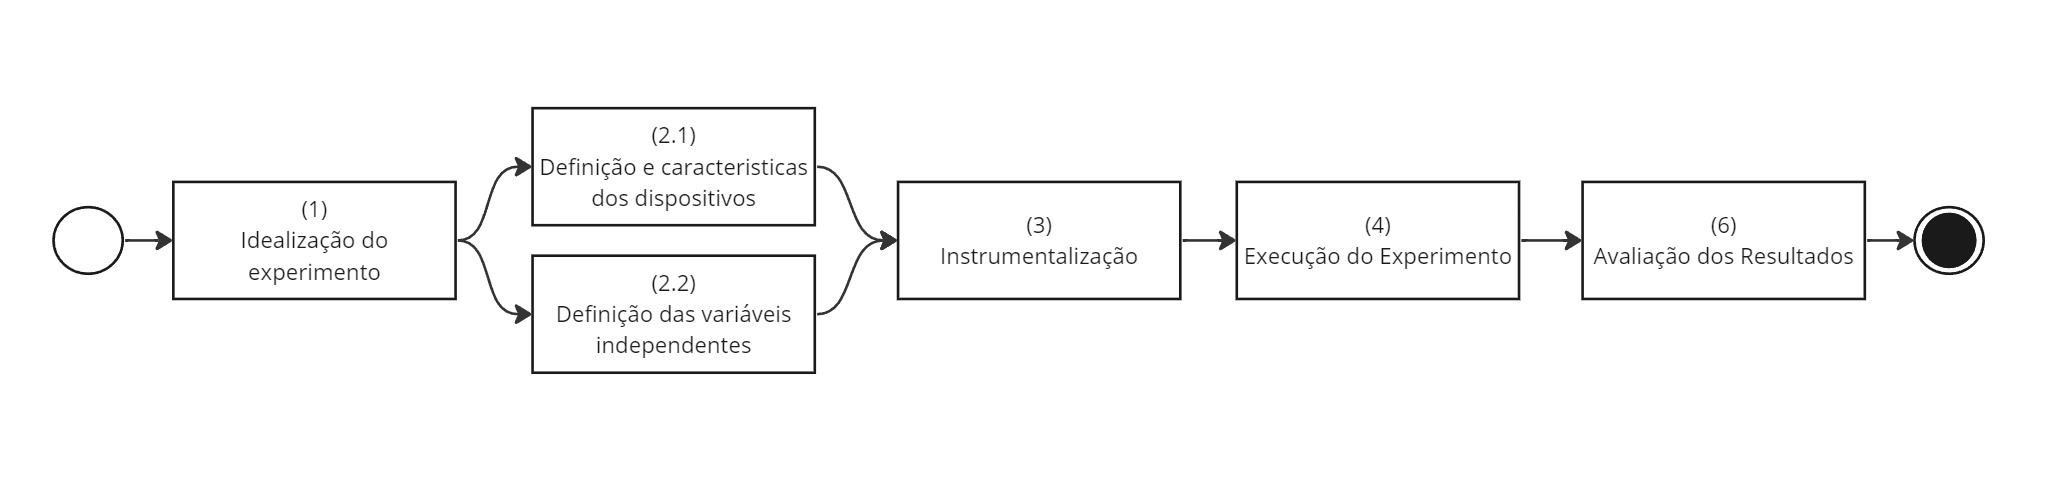
\includegraphics[width=1\linewidth]{Imagens/cap6/cap6metodologia.jpg}
	
	Fonte: elaborado pelo autor.
\end{figure} 


\section{Metodologia}

O experimento pretende comparar os efeitos do mecanismo de \textit{throttling} em dispositivos com capacidade de coleta de energia, com foco em examinar a disponibilidade de cada um relacionada aos  aspectos energéticos, em condições semelhantes de energia e atuação.

Para tal, foi observado a influência do mecanismo de throttling por meio da atuação de limites definidos que pudessem alterar o comportamento de um dos participantes em consideração aos valores de energia coletada e reserva energética, suas alterações de comportamento em virtude da  auto-análise de suas capacidades a medida que a variação de energia disponível acontece. Assim, conforme a Figura \ref{fig:cap6metodologia} representa a Idealização do experimento como etapa 1.

Na i, foi necessário abstrair os elementos envolvidos dada necessidade de garantir equidade de condições para todos dispositivos simulados simultaneamente. Buscando isolamento e consistência, optou-se pelo uso da plataforma Docker<footnote> como agente facilitador, atendendo às restrições de encapsulamento para que cada aplicação e suas dependências estejam contidas. Assim, conforme observado na figura <DIAGRAMA DE BLOCO DO SISTEMA>, a manobra possibilitou que ambos os sistemas pudessem ser paralelamente estimulados e ainda assim tivessem seus recursos controlados e seus termos de operação garantidos (capacidade de processador, memória e disco). 

Sendo assim, a composição do experimento considera:  I - Dispositivos com capacidade de coleta e armazenamento de energia estão inseridos em um dado ambiente de simulação controlada; II - Os dispositivos sempre recebem o mesmo valor como coleta de energia; III - Os dispositivos têm seus ciclos de recarga sincronizados; IV - Os dispositivos participantes possuem a mesma capacidade de armazenamento de energia coletada; V - Os dispositivos são submetidos simultaneamente ao mesmo tipo e quantidade de solicitações, constituindo os ciclos de carga.

Uma vez submetidos as execuções, os resultados coletados para análise são: I - Medição dos valores energéticos na relação tempo e ciclo de carga; II - Quantidade de solicitações atendidas ou negadas; III - Valores mínimos de reserva energética atingidos. Tais resultados serão melhores descritos posteriormente e apresentam o escopo de comparação entre os elementos participantes.



Dispositivos Utilizados


O cenário experimentado simula a atuação de nodes em dado ambiente externo. Estes node são concebidos com capacidade de coletar energia do meio onde estão inseridos, esta energia é considerada como entrada energética para o funcionamento do node, também é possível armazenar parte do recurso energético coletado e, por fim, a capacidade de resposta com a aferição de um dado simbólico qualquer do meio quando solicitado. Este node é considerado provedor, a medida que atende solicitações de tais aferições.
 